\chapter{Mechanisms}
Having established positive and significant treatment effects of  experience on outcomes in the market for public construction projects, we seek to investigate how does experience operate in practice to produce improved outcomes in the treated firms. Our objective is to provide evidence of some of the changes that might have taken place within firms which could help to achieve a higher rate of success in the market.

We start presenting the following working hypothesis regarding the benefits of experience among firms. Each details one way in which a firm might have experienced improvements that led to increased success in the market. This chapter objective is to test fully or partially these hypothesis with the data we have avalaible.

First we present our hypothesis. Then, for each one, we present the data, empirical strategy and results obtained.

\begin{enumerate}
  \item{H1}: experience produces improvements in cost measures in the firm, keeping constant the type of project. This improvement in cost operates either via economies of scale, since after winning the project the firm is bigger than before; or via adjustments in the production function itself, for example, by changing the relative inputs to produce.
  \item{H2}: experience allows the firm to produce at a higher quality than before, constant the cost of the works. This improvement operates because the firm, having performed certain tasks once, is able to better predict potential problems. Note that in the bidding phase this could be reflected in a better proposals.
  \item{H3}: experience increases the pool of projects that a firm can perform. Experience can allow the firm to produce either bigger or more complex projects, due to increased human and organizational capital.
\end{enumerate}

Our first can be easily studied because or main dataset of interest includes bid amounts. we can investigate the second hypothesis pa

The following sections study these hypothesis.

\section{Bids and experience}
This section investigates whether experience causes improvements in cost measures for treated firms. We do this by examining how do firm's bids evolve after the firm has been treated, i.e. after it has more experience. We assume that bid amounts are a non-decreasing function of bids' costs. This seems like a plausible assumption given previous investigations that have established this correlation, e.g. .

The relationship between bids and several firms characteristics has been investigated several times in the construction and economics literature. Relevant to the current investigation, we first mention.

The next section details briefly the data, empirical strategy and results, since most of the the empirical strategy and data is analogous to the analysis performed in the previous chapter.

\subsection{Data}
Our base dataset is the same as in the previous chapter, i.e a set of bids submitted by firms in auctions for public construction projects. However, instead of aggregating firm's experience and outcomes in time slices, our observations will be the bids themselves, so we keep the original unit of observation for outcomes. We still employ aggregation to compute experience at each point in time for every firm. As before, we filter those contracts where experience is not employed in the awarding factors.

Furthermore, we filter the first year in the data for our regression sample, since all firms have zero experience at this point and keeping it would introduce noise in the estimates do to treatments set to zero artificially. We do however employ all the avalaible years in the data to compute experience, as in the previous section.

Our data includes two key variables: bid amounts and a government estimate of the project. This estimate is prepared by the government unit in charge of the auction. It is of interest for the government to produce a reasonable estimate, since if the winning bid is below a certain fraction of this estimate, the government unit must undergo additional administrative steps to justify the awarding decision. The government estimate is avalaible in approximately of the projects in our sample.

We produce comparable bid amounts by dividing the bid amount by the corresponding government estimate to produce (arguably) comparable bids across different contracts which we call standarized bid. This procedure also helps to prevents some heteroskedastic effects and also reflects the most effects in our regression are expected to act "per-dollar" of a contract. We filter from the dataset standarized bids of less than 0.1 and over 5.0, since they could correspond to outlier cases and not to a regular auctioning procedure or project, or could show a very bad initial estimate from the government. This only eliminates 217 contracts. We do however use these contracts however to compute previous experience.

Figure \ref{fig:plot_bids_standarized} show a histogram of standarized bid amounts (we only show the interval  for convenience).

\begin{figure}
  \centering
  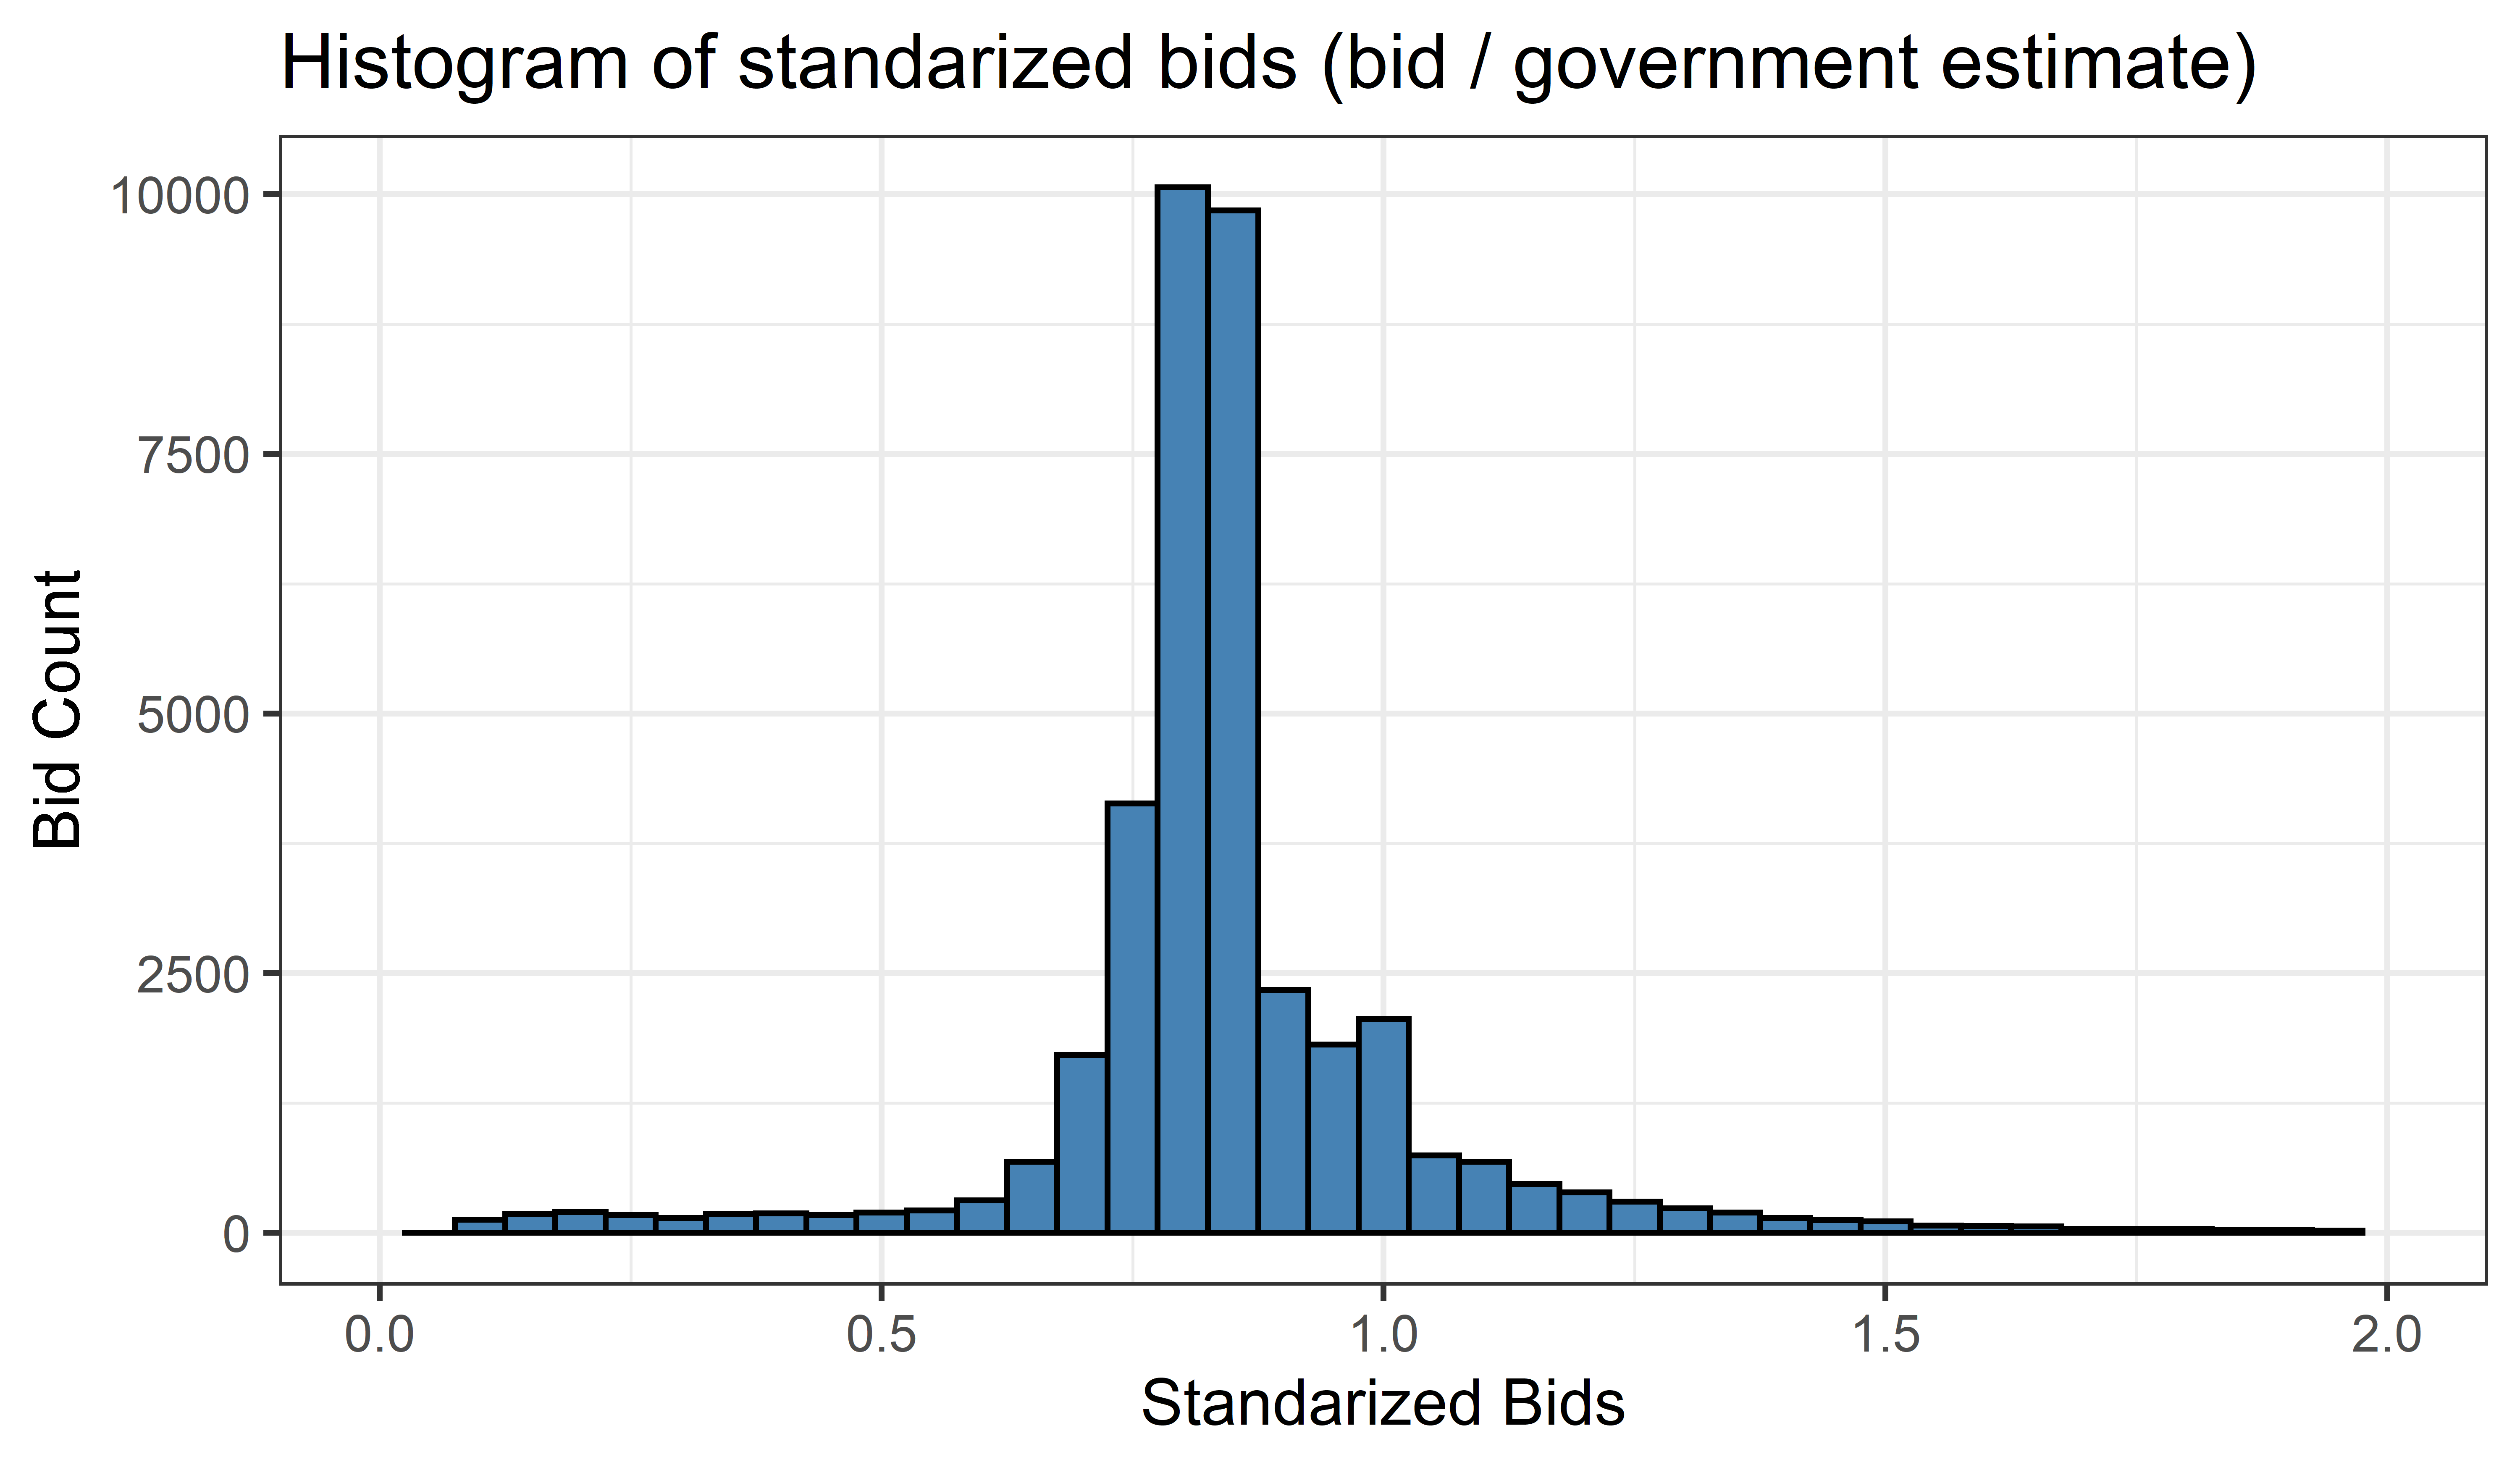
\includegraphics[scale=0.65]{plot_bids_standarized.png}
  \caption{Histogram of standarized bids}
  \label{fig:plot_bids_standarized}
\end{figure}

Table shows descriptive statistics of the bids employed in the analysis sample and of acecptance rates by the amount of experience.


\subsection{Empirical Strategy}
In this section, our main strategy is perform a regression of the form:

 Here, the outcome variable is a binary indicator which is 1 if the firm $i$ won the project $j$ at time $t$ and zero if not. Our treatment variable is experience, either in binary form $EXP>0$ or linear form $EXP$. We compute experience by summing all won up to $t$. Note that each row of our main dataset is an observation in the regression.
 %We employ an annualized form of experience to prevent overweighting the initial firms in the data.
Similarly as before, we have unobserved cost variables, specific to each firm, which might skew estimates upwards. The same argument employed in the previous chapter, regarding endogeneity of cost measures, can be applied in the case of equation.

We use the same strategy as before to produce consisten estimates, employing closely won bids to produce random variation in total experience. Table shows a comparison of contracts identified as close wins againts the rest of the sample. Note that there are very small modifications with respect to table , given the extra filtering steps employed in this section. The parameters employed in each IV strategy are also the same as the previous section.

We perform four regressions. The first two are OLS regressions and the second two are IV regressions, employing closely won contracts to instrument total experience. For each type, we develop one regression where the treatment is the binarye of previous experience and the second is total past experience.

\subsection{Results}

We show graphical results in Figure \ref{fig: plotbids_panel}

\begin{figure}
  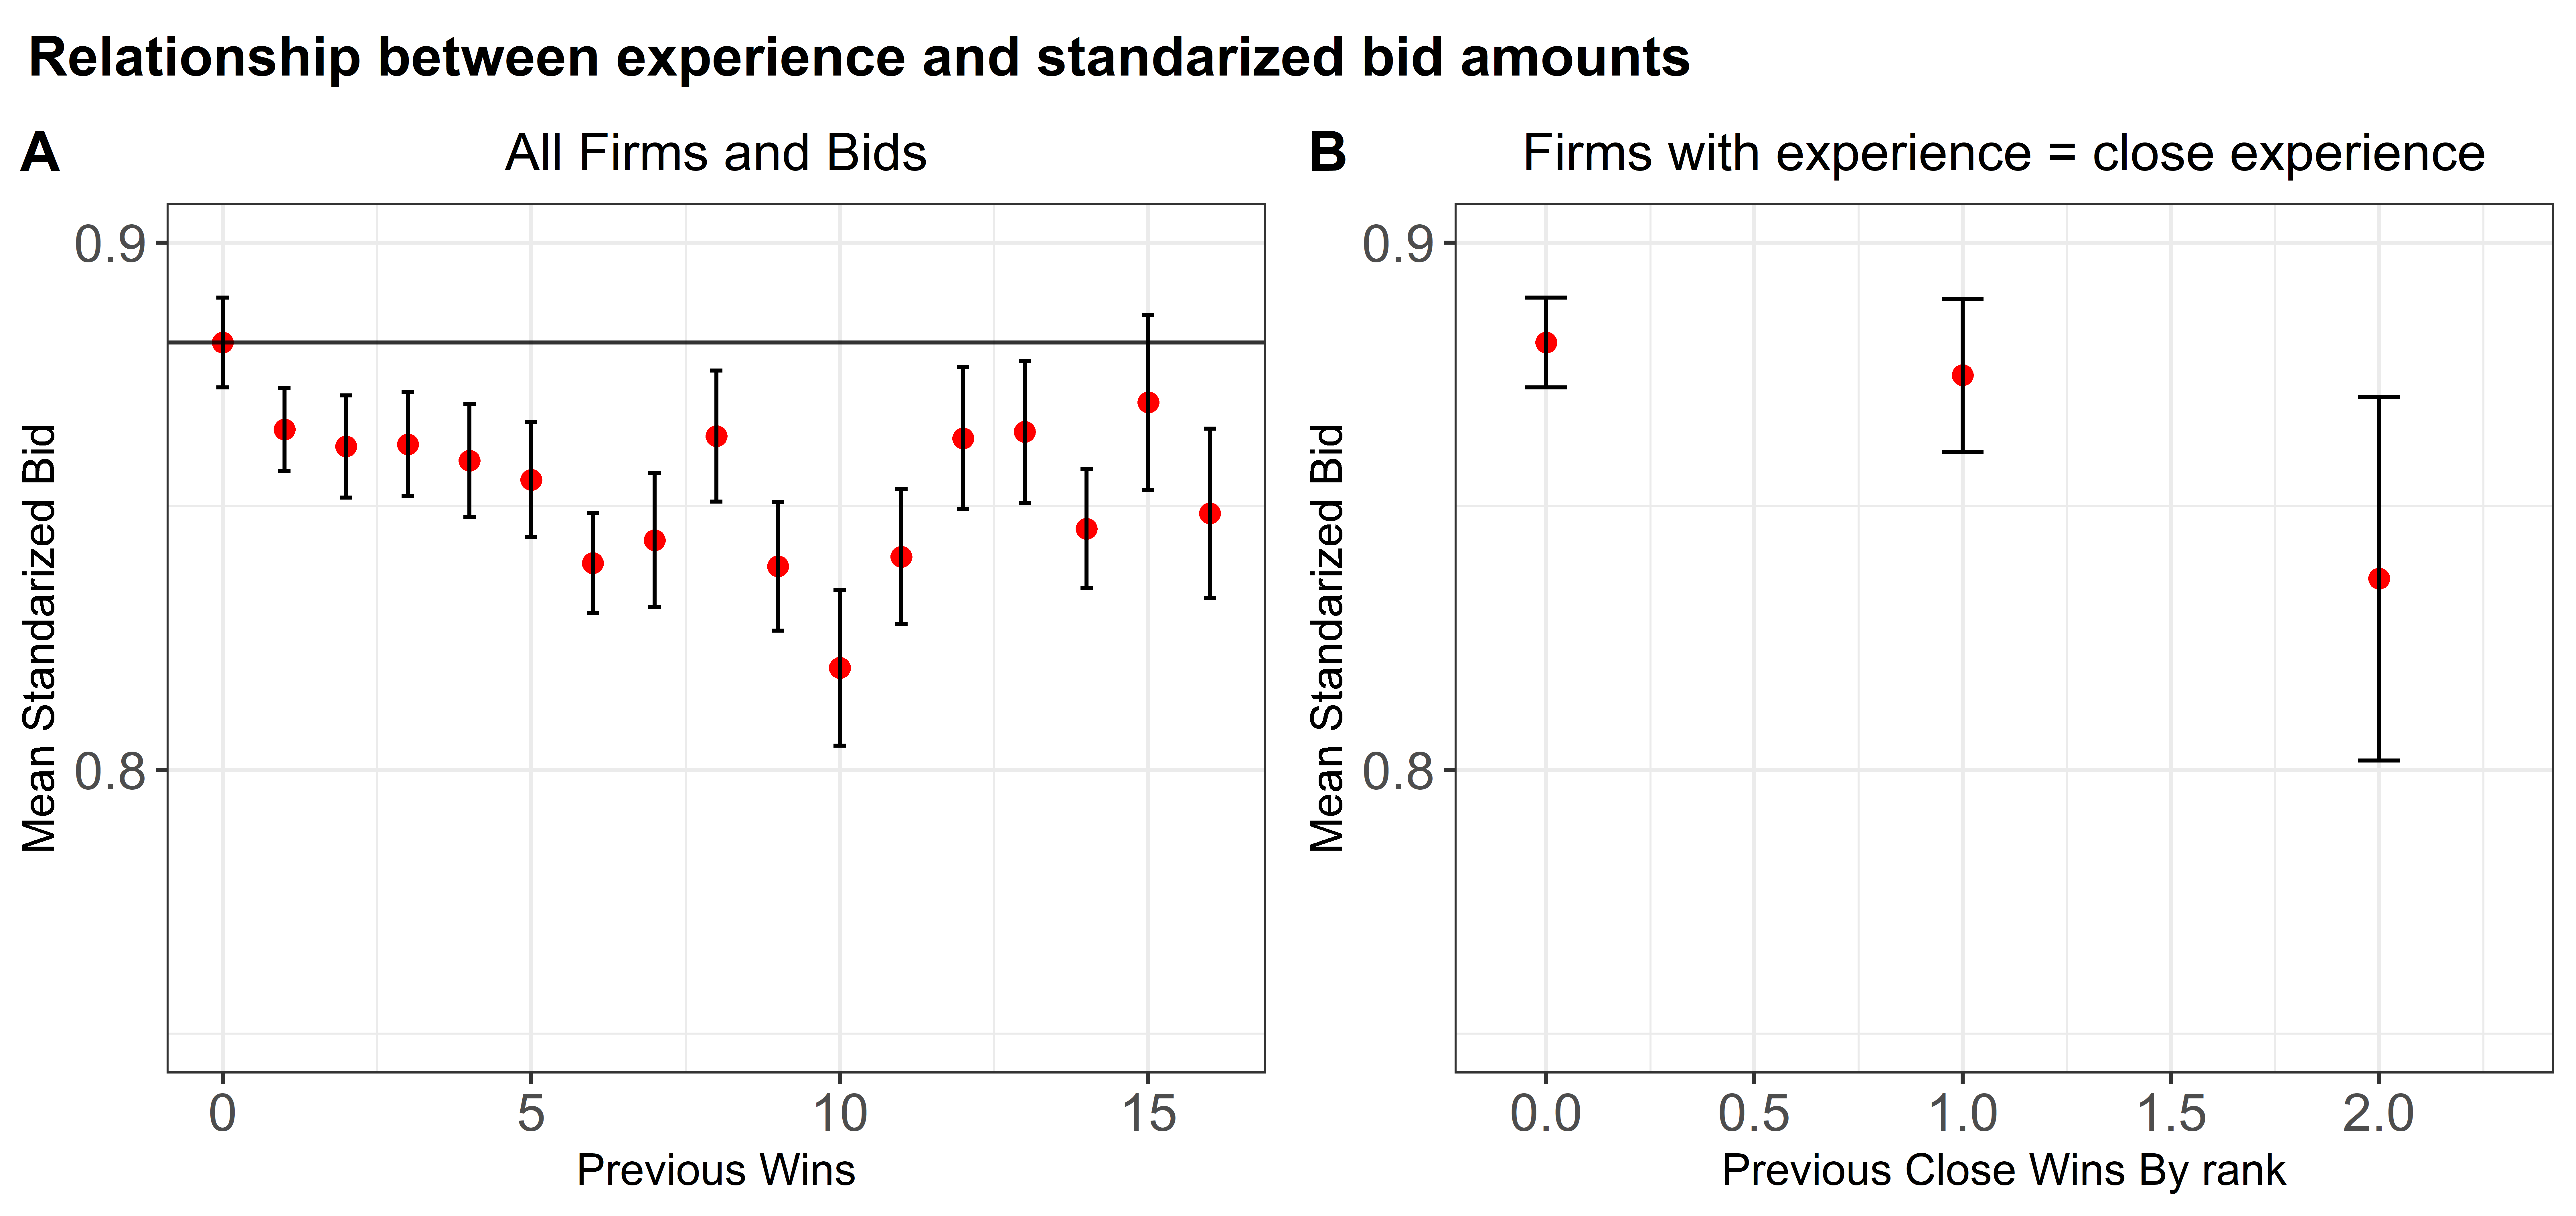
\includegraphics[scale=0.65]{plotbids_panel.png}
  \caption{Relationship between experience and standarized bid amounts}
  \label{fig: plotbids_panel}
\end{figure}



Table \ref{tab:table_bids_1} presents our main results.

\input{C:/repos/learn-doing/thesis/tables/table_bids_1.txt}


%%%%%%%%%%%%%%%%%%%%%%%%%%%%%%%%%%%%%%%%%%%%%%%%%%%%%%%%%%%%%%%%%%%%%%%%%%%%%%%%%%%%%%%%%%%%%%%%%%%

\section{Quality and Experience}
In order to test hypothesis number two, in this section we study if experience treatments causes firms to submit higher quality proposals. We do this by employing a step in the auctioning process aimed at controlling some basic quality conditions of a proposals, namely, formal requirements and qualifications.

Note that quality is explicitly evaluated in many contracts by including an item in the awarding criteria labeled as "technical specifications" or just "quality of the proposal". Our estimation is that around \% include some measure of technical evaluation in the awarding criteria.  Ideally, we would test the hypothesis that experience improves the quality of a firm's proposals by employing the score that each firm obtained in the technical or quality item of the evaluation criteria of the project. However, since our data has not this item avalaible by firm, we employ an alternative strategy,which focuses on measuring quality across a different but related dimension: the formal acceptance rate of the proposals.

Recall that, for each auction, firm proposals are analyzed in two steps. The first step only examines if the proposal fulfills all the formal requirements in the process. Formal requirements include the inclusion of legal documents, submitting each of the technical documents asked for in the bidding documents, etc. In essence, the first stage verifies that all proposals can be evaluated at an equal footing and that minimum bidding legal requirements are fulfilled. Clearly, whether a proposal was accepted is a measure of its quality, albeit an imperfect one. Altough it leaves out a significant part of the variation that would be expected in proposal's qualities, it is nonetheless an interesting measure of quality because formal acceptance is a necessary condition to win a project.

Our research design, detailed below, will test whether experienced firms have a higher formal acceptance rate than unexperienced firms at the formal revision step of the procuurement process. To our knowledge, ity has not been studied in the previous literature factors infleuencing formal acceptance of bid proposals.

\subsection{Data}
We employ our bid dataset similarly as the previous section. Each observation is a bid submitted by a firm to an auction held by the government. Since we are analyzing the formal revision part of the auction, and not scoring itself, we think that on principle we could skip the filtering of contracts that do include experience as an awarding factor. However, due to possible self-selection, we will examine both possibilities. We again filter the first year of the data in our analysis sample to prevent confounding effects.

We show some descriptive statistics of acceptance rates in table and Figure \ref{fig:plot_acceptance_rates}. We can already see that the fraction of firms getting all proposals rejected decreases with more than one proposal, which could be either due to revealed preferences or to the effect of learning about formal requirements after the first completed bidding process.

\begin{figure}
  
\includegraphics[scale=0.50]{plot_acceptance_rates.png}
  \caption{Acceptance rate for proposals sent by firms to auctions for public construction project.}
  \label{fig:plot_acceptance_rates}
\end{figure}

We end up with a dataset where each observation is a bid submitted by a firm to an auction of a public construction project, which includes as variables of interest wether the proposal was formally accepted, the experience of the firm at the time of the auction (both regular, annualized and close wins), and several  auxiliary variables that characterize the contract itself.

\subsection{Empirical Strategy}
We test wether experience leads to a higher rate of formal proposal acceptance employing the following regression:

Here, is and indicator variable that equals 1 if the firms' $i$ proposal for contract $j$ at time $t$ was accepted and zero if it was not. $EXP$ is our treatment variable, both in binary and linear functional forms. $X_{j}$ is a set of contract-specific controls, which include year, region, and the government body in charge of the auction. We include the controls for the possibility that government units in different  geographical regions have different levels of stringency when evaluating proposals for similar projects.

We are less worried about endogeneity with unobserved cost factors since formal revision does not relate to economic aspects of the proposal. However, it is possible that there are different levels of baseline levels of proposal-makeing abilities among firms, so we repeat our usual instrumentation of experience with close wins.

We perform four regressions. The first two are OLS regressions and the second two are IV regressions, employing closely won contracts to instrument total experience. For each type, we develop one regression where the treatment is the binary of previous experience and the second is annualized past experience.

\subsection{Results}
\begin{figure}
  \includegraphics[scale=0.65]{plot_acceptance_results.png}
  \caption{Acceptance rate for proposals sent by firms to auctions for public construction project.}
  \label{fig:plot_acceptance_results}
\end{figure}

\input{C:/repos/learn-doing/thesis/tables/table_acceptance_1.txt}
